\documentclass{article}

\usepackage{tikz} 
\usetikzlibrary{automata, positioning, arrows} 

\usepackage{amsthm}
\usepackage{amsfonts}
\usepackage{amsmath}
\usepackage{amssymb}
\usepackage{fullpage}
\usepackage{color}
\usepackage{parskip}
\usepackage{hyperref}
\usepackage{float}
\usepackage{forest}

\usepackage[section]{placeins}
  \hypersetup{
    colorlinks = true,
    urlcolor = blue,
    linkcolor= blue,
    citecolor= blue,
    filecolor= blue,
    }
    
\usepackage{listings}
\usepackage[utf8]{inputenc}                                                    
\usepackage[T1]{fontenc}                                                       

\definecolor{dkgreen}{rgb}{0,0.6,0}
\definecolor{gray}{rgb}{0.5,0.5,0.5}
\definecolor{mauve}{rgb}{0.58,0,0.82}

\lstset{frame=tb,
  language=haskell,
  aboveskip=3mm,
  belowskip=3mm,
  showstringspaces=false,
  columns=flexible,
  basicstyle={\small\ttfamily},
  numbers=none,
  numberstyle=\tiny\color{gray},
  keywordstyle=\color{blue},
  commentstyle=\color{dkgreen},
  stringstyle=\color{mauve},
  breaklines=true,
  breakatwhitespace=true,
  tabsize=3
}

\newtheoremstyle{theorem}
  {\topsep}   % ABOVESPACE
  {\topsep}   % BELOWSPACE
  {\itshape\/}  % BODYFONT
  {0pt}       % INDENT
  {\bfseries} % HEADFONT
  {.}         % HEADPUNCT
  {5pt plus 1pt minus 1pt} % HEADSPACE
  {}
\theoremstyle{plain} 
   \newtheorem{theorem}{Theorem}[section]
   \newtheorem{corollary}[theorem]{Corollary}
   \newtheorem{lemma}[theorem]{Lemma}
   \newtheorem{proposition}[theorem]{Proposition}
\theoremstyle{definition}
   \newtheorem{definition}[theorem]{Definition}
   \newtheorem{example}[theorem]{Example}
\theoremstyle{remark}    
  \newtheorem{remark}[theorem]{Remark}

\title{CPSC-354 Report}
\author{Ethan Tapia  \\ Chapman University}

\date{\today} 

\begin{document}

\maketitle

\begin{abstract}
\end{abstract}

\setcounter{tocdepth}{3}
\tableofcontents

\section{Introduction}\label{intro}

\section{Week by Week}\label{homework}

% =========================
% Week 1 
% =========================
\subsection{Week 1}

\textbf{Lecture Summary}

We introduced \emph{formal systems} and worked with Hofstadter’s MIU-system as a rule–based rewriting game.  
Alphabet: $\Sigma=\{M,I,U\}$.  
Axiom (start string): $MI$.  
Production rules:
\begin{enumerate}
    \item[\textbf{(R1)}] If a string ends in $I$, append $U$: $xI \Rightarrow xIU$.
    \item[\textbf{(R2)}] If a string is $Mx$, duplicate $x$: $Mx \Rightarrow Mxx$.
    \item[\textbf{(R3)}] Replace any $III$ by $U$: $xIIIy \Rightarrow xUy$.
    \item[\textbf{(R4)}] Delete any $UU$: $xUUy \Rightarrow xy$.
\end{enumerate}
Key idea: reason about \emph{invariants} that rules preserve, instead of searching blindly through derivations.

\bigskip
\textbf{Homework: The MU-puzzle}

\begin{definition}[I–count and residue]
For a string $w$, let $\#_I(w)$ be the number of $I$’s in $w$, and define the residue
\[
\varphi(w) \;=\; \#_I(w) \bmod 3 \in \{0,1,2\}.
\]
\end{definition}

\begin{lemma}[Effect of each rule on $\#_I$]\label{lem:rule-effects}
For any string $w$:
\begin{enumerate}
    \item \textbf{(R1)} and \textbf{(R4)} do not change $\#_I$.
    \item \textbf{(R2)} doubles the number of $I$’s \emph{after} the initial $M$, so $\varphi$ is multiplied by $2$ modulo $3$.
    \item \textbf{(R3)} decreases $\#_I$ by $3$, so $\varphi$ is unchanged.
\end{enumerate}
\end{lemma}

\begin{proposition}[Invariant modulo $3$]\label{prop:invariant}
Every string derivable from $MI$ has $\varphi\in\{1,2\}$. In particular, no derivable string has $\varphi=0$.
\end{proposition}

\begin{proof}
We use induction on the length of a derivation from $MI$.

\emph{Base.} $\varphi(MI)=1$.

\emph{Step.} Assume $\varphi\in\{1,2\}$ for some derivable $w$.  
By Lemma~\ref{lem:rule-effects}, rules (R1), (R3), and (R4) keep $\varphi$ unchanged, and rule (R2) maps $1\leftrightarrow 2$ modulo $3$. None of these operations yields $0$ from a value in $\{1,2\}$. Therefore the next string also has $\varphi\in\{1,2\}$.
\end{proof}

\begin{theorem}[MU is unreachable]
\label{thm:mu-unreachable}
$MU$ cannot be derived from $MI$ in the MIU-system.
\end{theorem}

\begin{proof}
$MU$ contains zero $I$’s, hence $\varphi(MU)=0$. By Proposition~\ref{prop:invariant}, every derivable string has residue $1$ or $2$. Thus $MU$ is not derivable.
\end{proof}

\textit{Conclusion.} Starting from $MI$ we can toggle the residue $1\leftrightarrow 2$ with (R2) and otherwise keep it fixed with (R1), (R3), (R4). We never reach residue $0$, so no sequence of legal rule applications yields $MU$.

\begin{center}
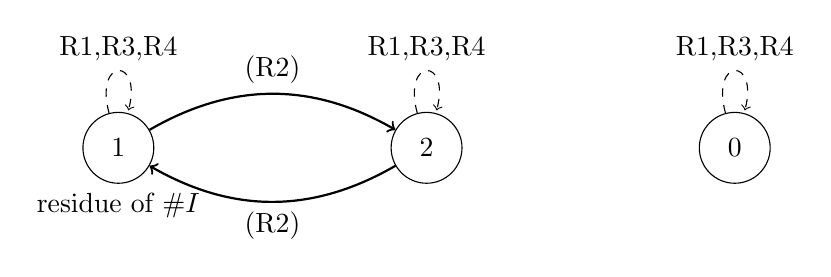
\begin{tikzpicture}[node distance=3cm, auto]
  \tikzstyle{state}=[circle,draw,minimum size=9mm]
  \node[state, label=below:{residue of $\#I$}] (Z1) {1};
  \node[state, right=of Z1] (Z2) {2};
  \node[state, right=of Z2] (Z0) {0};
  \path[->, thick]
    (Z1) edge[bend left] node[above]{(R2)} (Z2)
    (Z2) edge[bend left] node[below]{(R2)} (Z1);
  \path[->, dashed]
    (Z1) edge[loop above] node{R1,R3,R4} ()
    (Z2) edge[loop above] node{R1,R3,R4} ()
    (Z0) edge[loop above] node{R1,R3,R4} ();

\end{tikzpicture}
\end{center}
\textbf{Question:} If the MU-puzzle shows that some goals are unreachable due to invariants (like the mod-3 property of I’s), how does this idea connect to undecidability in programming languages?

\FloatBarrier

% =========================
% Week 2 
% =========================
\subsection{Week 2}

\textbf{Lecture Summary} \\
We introduced \emph{Abstract Reduction Systems (ARS)}: a pair $(A,R)$ with one-step reduction $R\subseteq A\times A$. Key notions:
reducible/normal form, joinability, confluence, termination, and unique normal forms.

\bigskip
\textbf{Homework Part 2: The 8 Combinations}

We provide an example ARS for each combination of
$(\text{confluent}, \text{terminating}, \text{unique NFs})$.
If a row is impossible, we explain why.

\begin{center}
\begin{tabular}{|c|c|c|l|}
\hline
\textbf{Confluent} & \textbf{Terminating} & \textbf{Unique NFs} & \textbf{Example} \\
\hline
True  & True  & True  & $A=\{a\},\ R=\emptyset$ (Fig.~\ref{fig:combo-ttt}) \\
True  & True  & False & \emph{Impossible} \\
True  & False & True  & $A=\{a,b\},\ R=\{(a,a),(a,b)\}$ (Fig.~\ref{fig:combo-tft}) \\
True  & False & False & $A=\{a\},\ R=\{(a,a)\}$ (Fig.~\ref{fig:combo-tff}) \\
False & True  & True  & \emph{Impossible} \\
False & True  & False & $A=\{a,b,c\},\ R=\{(a,b),(a,c)\}$ (Fig.~\ref{fig:combo-ftf}) \\
False & False & True  & \emph{Impossible} \\
False & False & False & $A=\{a,b,c\},\ R=\{(a,b),(a,c),(b,b),(c,c)\}$ (Fig.~\ref{fig:combo-fff}) \\
\hline
\end{tabular}
\end{center}

\noindent\textit{Why some rows are impossible.}
If an ARS has unique normal forms, it must be confluent.
If an ARS is both confluent and terminating, then every element reduces to a unique normal form.
Therefore the rows \((\text{T},\text{T},\text{F})\), \((\text{F},\text{T},\text{T})\), and \((\text{F},\text{F},\text{T})\) cannot occur.

\begin{figure}[H]
\centering
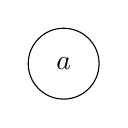
\begin{tikzpicture}[->,>=stealth',node distance=3cm,auto]
  \tikzstyle{obj}=[circle,draw,minimum size=9mm]
  \node[obj] (a) {$a$};
\end{tikzpicture}
\caption{Combination (True, True, True). Terminating, confluent, unique NF.}
\label{fig:combo-ttt}
\end{figure}

\begin{figure}[H]
\centering
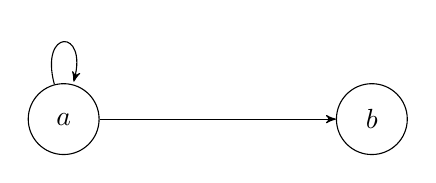
\begin{tikzpicture}[->,>=stealth',node distance=3cm,auto]
  \tikzstyle{obj}=[circle,draw,minimum size=9mm]
  \node[obj] (a) {$a$};
  \node[obj] (b) [right=of a] {$b$};
  \path (a) edge (b)
        (a) edge[loop above] (a);
\end{tikzpicture}
\caption{Combination (True, False, True). Non-terminating, confluent, unique NF $b$.}
\label{fig:combo-tft}
\end{figure}

\begin{figure}[H]
\centering
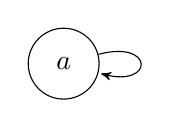
\begin{tikzpicture}[->,>=stealth',node distance=3cm,auto]
  \tikzstyle{obj}=[circle,draw,minimum size=9mm]
  \node[obj] (a) {$a$};
  \path (a) edge[loop right] (a);
\end{tikzpicture}
\caption{Combination (True, False, False). Non-terminating, confluent, no normal form.}
\label{fig:combo-tff}
\end{figure}

\begin{figure}[H]
\centering
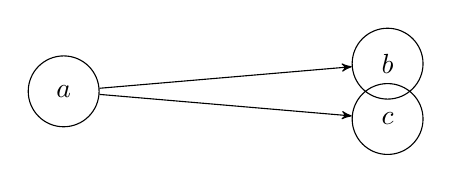
\begin{tikzpicture}[->,>=stealth',node distance=3.2cm,auto]
  \tikzstyle{obj}=[circle,draw,minimum size=9mm]
  \node[obj] (a) {$a$};
  \node[obj] (b) [right=of a,yshift=10pt] {$b$};
  \node[obj] (c) [right=of a,yshift=-10pt] {$c$};
  \path (a) edge (b)
        (a) edge (c);
\end{tikzpicture}
\caption{Combination (False, True, False). Terminating, not confluent; two distinct normal forms $b,c$ are not joinable.}
\label{fig:combo-ftf}
`\end{figure}

\begin{figure}[H]
\centering
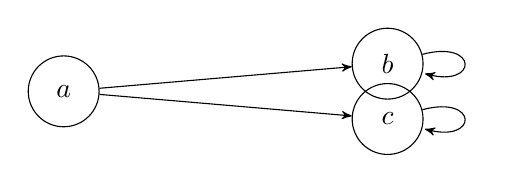
\begin{tikzpicture}[->,>=stealth',node distance=3.2cm,auto]
  \tikzstyle{obj}=[circle,draw,minimum size=9mm]
  \node[obj] (a) {$a$};
  \node[obj] (b) [right=of a,yshift=10pt] {$b$};
  \node[obj] (c) [right=of a,yshift=-10pt] {$c$};
  \path (a) edge (b)
        (a) edge (c)
        (b) edge[loop right] (b)
        (c) edge[loop right] (c);
\end{tikzpicture}
\caption{Combination (False, False, False). Non-terminating (loops), not confluent, no unique normal forms.}
\label{fig:combo-fff}
\end{figure}

\FloatBarrier

\noindent\paragraph{Conclusion.}
The MU-puzzle illustrates how invariants prove impossibility in a formal system.
The ARS framework provides the general language to study rewrite systems via termination, confluence, and normal forms.
The 8-combination analysis shows which behaviors are possible and which are structurally impossible.

\noindent\paragraph{Question:}
Could there be a general framework that unifies invariants with confluence and termination, so that impossibility and determinism appear as two sides of the same rewriting theory?
\subsection{Week 3}
\textbf{Lecture Summary}
\\TBD

\textbf{Homework 3}
\paragraph{Exercise 5}

Consider an ARS with
\[
A = \{a,b\}^* = \{\varepsilon, a, b, aa, ab, ba, bb, aaa, \dots \}
\]
and rewrite rules
\[
ab \to ba, \qquad 
ba \to ab, \qquad 
aa \to \varepsilon, \qquad 
b \to \varepsilon
\]

\begin{enumerate}
  \item \textbf{Reduce some example strings such as $abba$ and $bababa$.}
  \[
    abba \to aa \to \varepsilon, \qquad
    bababa \to aaa \to a
  \]

  \item \textbf{Find two strings that are not equivalent. How many non-equivalent strings can you find?}
  \begin{itemize}
    \item $\varepsilon$
    \item $a$
  \end{itemize}
  These have different normal forms and cannot be transformed into each other.

  \item \textbf{How many equivalence classes does $\stackrel{\ast}{\longleftrightarrow}$ have? What are the normal forms?} \\
  There are two equivalence classes:
  \begin{enumerate}
    \item Strings whose normal form is $\varepsilon$,
    \item Strings whose normal form is $a$.
  \end{enumerate}
  The class is determined by the parity of the number of $a$’s in the string.

  \item \textbf{Can you modify the ARS so that it becomes terminating without changing its equivalence classes?} \\
  Yes. Remove one of the first two rules. They only permute $a$ and $b$ and do not affect equivalence classes, but having both makes the system non-terminating.

  \item \textbf{Question:} \\
  If I remove all the $b$’s from a string, does the remaining word reduce to $a$ or to $\varepsilon$?  

  \textbf{Answer:} This can be answered using the ARS because $b \to \varepsilon$ always deletes $b$’s, and the final result depends only on whether the number of $a$’s left is odd or even. Odd $\mapsto a$, even $\mapsto \varepsilon$.
\end{enumerate}

\paragraph{Exercise 5b}

Now replace the rule $aa \to \varepsilon$ with $aa \to a$.

\begin{enumerate}
  \item \textbf{Reduce some example strings such as $abba$ and $bababa$.}
  \[
    abba \to aa \to a, \qquad
    bababa \to aaa \to aa \to a
  \]

  \item \textbf{Find two strings that are not equivalent.}
  \begin{itemize}
    \item $\varepsilon$
    \item $a$
  \end{itemize}

  \item \textbf{How many equivalence classes are there? What are the normal forms?} \\
  There are two equivalence classes:
  \begin{enumerate}
    \item Strings with no $a$’s $\mapsto$ normal form $\varepsilon$,
    \item Strings with at least one $a$ $\mapsto$ normal form $a$.
  \end{enumerate}

  \item \textbf{Modify the ARS to make it terminating.} \\
  As above, remove one of the two swapping rules $ab \leftrightarrow ba$.

  \item \textbf{Question:} \\
  Is the system confluent? That is, if a string can be reduced in two different ways, do the reductions always lead to the same normal form?
\end{enumerate}

\subsection{Week 4}
\textbf{Lecture Summary}
\\An \emph{invariant} is a function or property that remains unchanged under the rewriting relation of an ARS. 
They are central tools across science (e.g.\ conservation laws in physics, chemistry, and biology) and mathematics. 
Formally, $P:A\to B$ is an invariant if $a\to b \Rightarrow P(a)=P(b)$. 
Strong invariants preserve exact equality, while weak invariants preserve truth of properties. 
Invariants induce partitions on $A$, often serving as abstractions of the equivalence relation $\leftrightarrow^\ast$. 
They can be used to prove impossibility (show $P(a)=\text{true}$, $P(b)=\text{false}$) and to build \emph{complete invariants}, which fully classify equivalence classes. 
Examples include letter counts in string rewriting systems and parity arguments in puzzles (domino tilings, sliding puzzles). 
In programming, invariants explain correctness of while-loops and recursion, while measure functions guarantee termination.


\textbf{Homework 4.1}\\
\textbf{Algorithm}
\begin{verbatim}
while b != 0:
  temp = b
  b = a mod b
  a = temp
return a
\end{verbatim}

\paragraph{Conditions under which it always terminates.}
Assume \(a,b\in\mathbb{N}\) with \(b\ge 0\). If \(b=0\) the loop does not run and the program returns immediately. If \(b>0\) then each loop iteration is well defined and yields a strictly smaller nonnegative \(b\) because \(a \bmod b\in\{0,1,\dots,b-1\}\). Thus the loop must terminate. (Equivalently: Euclid’s algorithm terminates for all nonnegative integers, not both zero.)

\paragraph{Measure function and proof.}
Let the state be the pair \((a,b)\in\mathbb{N}^2\). Define
\[
\phi(a,b)=b.
\]
Suppose the guard holds, so \(b>0\). One loop step computes
\[
(a',b')=(b,\; a\bmod b).
\]
Then \(0\le b' < b\), hence \(\phi(a',b')=b' < b=\phi(a,b)\).
Therefore \(\phi\) strictly decreases on every iteration while staying in \(\mathbb{N}\). Since \(>\) on \(\mathbb{N}\) is well founded, no infinite descent exists, so the loop terminates.

\textbf{Homework 4.2}\\
\textbf{Fragment}
\begin{verbatim}
function merge_sort(arr, left, right):
  if left >= right:
    return
  mid = (left + right) / 2   // integer division
  merge_sort(arr, left, mid)
  merge_sort(arr, mid+1, right)
  merge(arr, left, mid, right)
\end{verbatim}

\paragraph{Claim.}
\(\displaystyle \phi(left,right)=right-left+1\) is a measure function for the recursive calls of \texttt{merge\_sort}.

\paragraph{Proof.}
We reason about the domain \(D=\{(l,r)\in\mathbb{Z}^2 \mid l\le r\}\) with the measure \(\phi(l,r)=r-l+1\in\mathbb{N}\).

If \(left\ge right\) then \(\phi(left,right)\in\{0,1\}\) and the function returns, so there is no recursive descent.

Assume \(left<right\). Let \(mid=\lfloor (left+right)/2\rfloor\). Standard bounds give
\[
left \le mid < right \quad\text{and}\quad left < mid+1 \le right.
\]
Hence both subranges are valid:
\[
(left,mid)\in D, \qquad (mid+1,right)\in D.
\]
Their measures satisfy
\[
\phi(left,mid)=mid-left+1 \le \left\lfloor\frac{left+right}{2}\right\rfloor-left+1
< \frac{left+right}{2}-left+1
= \frac{right-left+2}{2} \le right-left,
\]
so \(\phi(left,mid) \le right-left < right-left+1=\phi(left,right)\). Similarly,
\[
\phi(mid+1,right)=right-(mid+1)+1=right-mid
\le right-\left\lfloor\frac{left+right}{2}\right\rfloor
< right-\frac{left+right}{2}
= \frac{right-left}{2}
< right-left+1=\phi(left,right).
\]
Thus each recursive argument strictly decreases the measure \(\phi\). Since \(\phi\) takes values in \(\mathbb{N}\) and strictly decreases along every recursion chain, the recursion is well founded and \texttt{merge\_sort} terminates.

\textbf{Question:} \\
We can discovered that Euclid’s algorithm always stops. But how could you use an invariant to also show that it actually gives the greatest common divisor, not just any number?

\subsection{Week 5}
\textbf{Lecture Summary}\\
Lambda calculus is a minimal but Turing-complete language with only three constructs: abstraction ($\lambda x.e$ defines a function), application ($e_1\,e_2$ applies a function to an argument), and variables (simple names without assignment). Application associates to the left and abstraction chains naturally. Computation is substitution: $(\lambda x.M)\,N \rightsquigarrow M[N/x]$ (the $\beta$-rule), with bound variables freely renamable ($\alpha$-equivalence) to avoid capture. Functions can return functions (currying), and using Church encodings, numbers and arithmetic can be represented purely by substitution.


\textbf{Homework 5: Lambda Calculus Reduction}\\
\textbf{We Evaluate:}
\[
(\lambda f.\,\lambda x.\, f(f(x))) \; (\lambda f.\,\lambda x.\, f(f(f(x))))
\]
\noindent
\textbf{Step 1: Rename the boud variables of the second term to avoid clashes} 
\[
(\lambda f.\,\lambda x.\, f(f(x))) \; (\lambda g.\,\lambda y.\, g(g(g(y))))
\]

\noindent
\textbf{Step 2: Apply the outer function to its argument}
\[
\lambda x.\, (\lambda g.\,\lambda y.\, g(g(g(y)))) \big( (\lambda g.\,\lambda y.\, g(g(g(y))))\, x \big)
\]

\noindent
\textbf{Step 3: Reduce the inner application}
\[
\lambda x.\, (\lambda g.\,\lambda y.\, g(g(g(y)))) \, (\lambda y.\, x(x(xy)))
\]

\noindent
\textbf{Step 4: Apply again}
\[
\lambda x.\,\lambda y.\, (\lambda y.\, x(x(xy))) \big((\lambda y.\, x(x(xy))) \, ((\lambda y.\, x(x(xy)))\, y)\big)
\]

\noindent
\textbf{Step 5: Evaluate the nested calls}
\[
\lambda x.\,\lambda y.\, x(x(x(x(x(x(x(x(xy)))))))))
\]

\noindent
\textbf{Final result.} This is the Church numeral
\[
\lambda f.\,\lambda x.\, f^9(x)
\]
This is the number $9$ in Church encoding.

\medskip
\noindent
\emph{Note:} The workout shows that $2\,3 = 9$ for Church numerals. In general, Church numerals encode repeated function application, and application corresponds to multiplication.

\textbf{Question:} If variable names don’t matter in $\lambda$
-calculus, what does that suggest about how meaning can exist independently of representation?

\subsection{Week 6}

\textbf{Lecture Summary}\\  
This lecture introduced recursion in the $\lambda$-calculus via the \textit{fixed point combinator}. We learned that recursion can be encoded without special syntax by defining \texttt{fix} such that $\texttt{fix}\ F \to F(\texttt{fix}\ F)$. Using this, one can define recursive functions like factorial. We also reviewed the definitions of \texttt{let} and \texttt{let rec}, which expand into $\lambda$-abstractions and applications of \texttt{fix}. The key point is that recursion in functional languages comes from self-application and fixed points, with the famous $Y$-combinator as a canonical construction.

\textbf{Homework 6: Fixed Points and Recursion}\\

\textbf{Rules:}\\
\[
\begin{aligned}
\texttt{fix}\ F &\;\to\; F\,(\texttt{fix}\ F) \qquad &\textbf{(def of fix)}\\
\texttt{let}\ x=e_1\ \texttt{in}\ e_2 &\;\to\; (\lambda x.\,e_2)\ e_1 \qquad &\textbf{(def of let)}\\
\texttt{let rec}\ f=e_1\ \texttt{in}\ e_2 &\;\to\; \texttt{let}\ f=(\texttt{fix}\ (\lambda f.\,e_1))\ \texttt{in}\ e_2 \qquad &\textbf{(def of let rec)}
\end{aligned}
\]

\textbf{Abbreviation.}  
For readability set
\[
G \;\equiv\; \lambda f.\,\lambda n.\, \texttt{if}\ n=0\ \texttt{then}\ 1\ \texttt{else}\ n * f(n-1).
\]

\textbf{Goal term.}
\[
\texttt{let rec}\ \texttt{fact} = \lambda n.\, \texttt{if}\ n=0\ \texttt{then}\ 1\ \texttt{else}\ n * \texttt{fact}(n-1)\ \texttt{in}\ \texttt{fact}\ 3
\]

\textbf{Derivation}
\[
\begin{aligned}
&\texttt{let rec}\ \texttt{fact} = \lambda n.\,\texttt{if}\ n=0\ \texttt{then}\ 1\ \texttt{else}\ n * \texttt{fact}(n-1)\ \texttt{in}\ \texttt{fact}\ 3
\\
\to\;& \texttt{let}\ \texttt{fact} = \texttt{fix}\,G\ \texttt{in}\ \texttt{fact}\ 3 \quad \textbf{\small<def of let rec>}
\\
\to\;& (\lambda \texttt{fact}.\, \texttt{fact}\ 3)\ (\texttt{fix}\,G) \quad \textbf{\small<def of let>}
\\
\to\;& (\texttt{fix}\,G)\ 3 \quad \textbf{\small<}\beta\textbf{-rule>}
\\
\to\;& (G(\texttt{fix}\,G))\ 3 \quad \textbf{\small<def of fix>}
\\
\to\;& (\lambda n.\, \texttt{if}\ n=0\ \texttt{then}\ 1\ \texttt{else}\ n*(\texttt{fix}\,G)(n-1))\ 3 \quad \textbf{\small<}\beta\textbf{-rule>}
\\
\to\;& \texttt{if}\ 3=0\ \texttt{then}\ 1\ \texttt{else}\ 3 * (\texttt{fix}\,G)(2) \quad \textbf{\small<}\beta\textbf{-rule>}
\\
\to\;& 3 * (\texttt{fix}\,G)(2) \quad \textbf{\small<def of if>}
\\
\to\;& 3 * \big(G(\texttt{fix}\,G)\big)\ 2 \quad \textbf{\small<def of fix>}
\\
\to\;& 3 * (\lambda n.\,\texttt{if}\ n=0\ \texttt{then}\ 1\ \texttt{else}\ n*(\texttt{fix}\,G)(n-1))\ 2 \quad \textbf{\small<}\beta\textbf{-rule>}
\\
\to\;& 3 * (\texttt{if}\ 2=0\ \texttt{then}\ 1\ \texttt{else}\ 2*(\texttt{fix}\,G)(1)) \quad \textbf{\small<}\beta\textbf{-rule>}
\\
\to\;& 3 * (2 * (\texttt{fix}\,G)(1)) \quad \textbf{\small<def of if>}
\\
\to\;& 3 * (2 * (G(\texttt{fix}\,G))\ 1) \quad \textbf{\small<def of fix>}
\\
\to\;& 3 * (2 * (\lambda n.\,\texttt{if}\ n=0\ \texttt{then}\ 1\ \texttt{else}\ n*(\texttt{fix}\,G)(n-1))\ 1) \quad \textbf{\small<}\beta\textbf{-rule>}
\\
\to\;& 3 * (2 * (\texttt{if}\ 1=0\ \texttt{then}\ 1\ \texttt{else}\ 1*(\texttt{fix}\,G)(0))) \quad \textbf{\small<}\beta\textbf{-rule>}
\\
\to\;& 3 * (2 * (1 * (\texttt{fix}\,G)(0))) \quad \textbf{\small<def of if>}
\\
\to\;& 3 * (2 * (1 * (G(\texttt{fix}\,G))\ 0)) \quad \textbf{\small<def of fix>}
\\
\to\;& 3 * (2 * (1 * (\lambda n.\,\texttt{if}\ n=0\ \texttt{then}\ 1\ \texttt{else}\ n*(\texttt{fix}\,G)(n-1))\ 0)) \quad \textbf{\small<}\beta\textbf{-rule>}
\\
\to\;& 3 * (2 * (1 * (\texttt{if}\ 0=0\ \texttt{then}\ 1\ \texttt{else}\ 0*(\texttt{fix}\,G)(-1)))) \quad \textbf{\small<}\beta\textbf{-rule>}
\\
\to\;& 3 * (2 * (1 * 1)) \quad \textbf{\small<def of if>}
\\
\to\;& 3 * (2 * 1) \quad \textbf{\small<arith>}
\\
\to\;& 3 * 2 \quad \textbf{\small<arith>}
\\
\to\;& 6 \quad \textbf{\small<arith>}
\end{aligned}
\]

\textbf{Result:} \texttt{fact 3} reduces to $6$, each step justified by \textbf{def of let rec}, \textbf{def of let}, \(\beta\)\textbf{-rule}, \textbf{def of fix}, \textbf{def of if}, and \textbf{arith}.

\textbf{Question:} Since the fixed point combinator allows functions to call themselves without being named, what does this suggest about the nature of recursion and whether naming is essential for defining self-reference?

\subsection{Week 7}\\
\textbf{Lecture Summary}\\
This lecture introduced parsing and context-free grammars (CFGs) using the calculator example. Parsing was explained as the process of turning concrete syntax (strings) into abstract syntax (trees). We saw how CFG rules capture precedence and associativity, and how parse trees differ from simplified abstract syntax trees (ASTs). Lisp was discussed as a language where programmers essentially write abstract syntax directly. \\

\textbf{Homework: Parse Trees for Arithmetic Expressions}

\textbf{1. Expression: $2+1$}

\begin{forest}
[Exp
  [Exp
    [Exp1
      [Exp2
        [Integer [2]]]]]
  [+]
  [Exp1
    [Exp2
      [Integer [1]]]]]
\end{forest}

\textbf{2. Expression: $1+2*3$}

\begin{forest}
[Exp
  [Exp
    [Exp1
      [Exp2
        [Integer [1]]]]]
  [+]
  [Exp1
    [Exp1
      [Exp2 [Integer [2]]]]
    [*]
    [Exp2 [Integer [3]]]]]
\end{forest}

\textbf{3. Expression: $1+(2*3)$}

\begin{forest}
[Exp
  [Exp
    [Exp1
      [Exp2
        [Integer [1]]]]]
  [+]
  [Exp1
    [Exp2
      [(]
        [Exp
          [Exp1
            [Exp1
              [Exp2 [Integer [2]]]]
            [*]
            [Exp2 [Integer [3]]]]]
      [)]]]]
\end{forest}

\textbf{4. Expression: $(1+2)*3$}

\begin{forest}
[Exp
  [Exp1
    [Exp1
      [Exp2
        [(]
          [Exp
            [Exp
              [Exp1
                [Exp2 [Integer [1]]]]]
            [+]
            [Exp1
              [Exp2 [Integer [2]]]]]
        [)]]]
    [*]
    [Exp2 [Integer [3]]]]]
\end{forest}


\textbf{5. Expression: $1+2*3+4*5+6$}

\begin{forest}
[Exp
  [Exp
    [Exp
      [Exp1 [Exp2 [Integer [1]]]]
      [+]
      [Exp1
        [Exp1 [Exp2 [Integer [2]]]]
        [*]
        [Exp2 [Integer [3]]]]]
    [+]
    [Exp1
      [Exp1 [Exp2 [Integer [4]]]]
      [*]
      [Exp2 [Integer [5]]]]]
  [+]
  [Exp1
    [Exp2 [Integer [6]]]]]
\end{forest}

\textbf{Question:} If Lisp lets programmers write abstract syntax directly, what does this reveal about the trade-offs between readability for humans and ease of parsing for machines?

\subsection{Week 8}
\textbf{Lecture Summary}

This lecture introduced formal proofs in Lean using the natural numbers tutorial world. We practiced rewriting with lemmas such as \texttt{add\_zero} and \texttt{add\_succ}, and learned how to control which occurrence gets rewritten. The exercises illustrated how even simple arithmetic like $2 + 2 = 4$ requires careful step-by-step rewriting when starting from the axioms of Peano arithmetic. The key insight is that Lean forces us to be explicit about each rule application, which deepens our understanding of how proofs are built from small definitional steps.

\textbf{Homework 8: Lean Tutorial World (Levels 5--8)}

\textit{Level 5.} Prove $a + (b + 0) + (c + 0) = a + b + c$.

\begin{verbatim}
rw [add_zero c]
rw [add_zero]
rfl
\end{verbatim}

\textit{Level 6.} Prove $succ n = n + 1$.

\begin{verbatim}
rw [one_eq_succ_zero]
rw [add_succ]
rw [add_zero]
rfl
\end{verbatim}

\textit{Level 7.} Prove $2 + 2 = 4$.

\begin{verbatim}
rw [two_eq_succ_one]
rw [add_succ]
rw [one_eq_succ_zero]
rw [add_succ]
rw [add_zero]
rw [four_eq_succ_three]
rw [three_eq_succ_two]
rw [two_eq_succ_one]
rw [one_eq_succ_zero]
rfl
\end{verbatim}

\textit{Level 8 (alternative short proof).} Another valid solution using \texttt{nth\_rewrite} and reversed rewrites.

\begin{verbatim}
nth_rewrite 2 [two_eq_succ_one]
rw [add_succ]
rw [one_eq_succ_zero]
rw [add_succ, add_zero]
rw [← three_eq_succ_two]
rw [← four_eq_succ_three]
rfl
\end{verbatim}

\textbf{Question:} When Lean forces us to spell out each small step (like showing $2 + 2 = 4$ from the Peano axioms), it reveals how much structure is hidden in even basic arithmetic. What does this suggest about the trade-off between human mathematical intuition (where $2 + 2 = 4$ is obvious) and machine-checked rigor (where nothing is obvious until proved)?




\section{Evidence of Participation}

\section{Conclusion}\label{conclusion}

\begin{thebibliography}{99}
\bibitem[BLA]{bla} Author, \href{https://en.wikipedia.org/wiki/LaTeX}{Title}, Publisher, Year.
\end{thebibliography}

\end{document}
